\documentclass[doctor,review,color]{buaa}

\begin{document}

% Info
\thesistilte{\textcolor{red}{请在此处写各位同学的论文题目}}
\title{\buaaatthesistitle}
\authorname{研究生姓名}
\author{\buaaatauthorname}
\tutor{导师姓名}
\stuno{XXXX}
\major{专业名称}
\direction{研究方向}

% Title_page(封面)
\pdfbookmark[0]{\buaaatthesistitle}{cover}
\maketitle
\linespread{1.5}
\pagestyle{frontmatter}

% Toc(目录)
\newpage
\phantomsection
\pdfbookmark[section]{\contentname}{contents}
\tableofcontents
\newpage
\phantomsection
\pdfbookmark[section]{\figurecontentname}{lof}
\listoffigures
% 模板暂无表格
%\newpage
%\phantomsection
%\pdfbookmark[section]{\tablecontentname}{lot}
%\listoftables
\newpage
\pagestyle{mainmatter}

% Main content
\section{研究方向概述}
简要介绍论文研究方向主要研究分支,每个分支做了哪方面的研究

\begin{figure}[h]
	\centering
	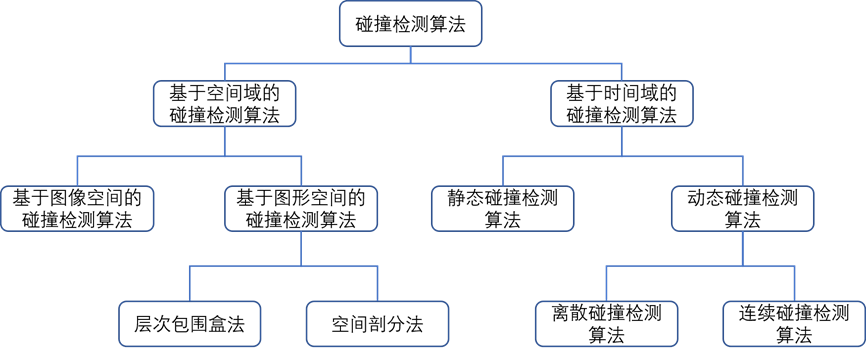
\includegraphics[width=\linewidth]{fig_direction}
	\caption{碰撞检测算法分类}
\end{figure}

\section{国内外研究现状}
详细介绍各分支的理论、方法或技术研究现状

\subsection{XXX研究现状}
XXX研究现状
\subsection{XXX研究现状}
XXX研究现状
\subsection{XXX研究现状}
XXX研究现状
\section{研究现状总结与分析}
\subsection{论文研究领域存在的问题}
论文研究领域存在哪些尚未解决的问题   
\subsection{论文研究领域的发展趋势}
论文研究方向的未来发展趋势
\subsection{研究现状分析结论}
描述哪些问题是本论文需要解决的


% References
\clearpage
\nocite{*}
\phantomsection
\addcontentsline{toc}{section}{\bibname}
\bibliography{Refs}

\end{document}